\documentclass[crop=false, class=book]{standalone}

\usepackage{lipsum}

\begin{document}
	\section{GCE}
	Il programma \textit{GCE} permette di modellare la distribuzione dei k-mer presenti nei dati sequenziati e di stimare la dimensione del genoma, le sequenze ripetitive e il rapporto di eterozigosi~\cite{liu2013GCE}. Il programma è open-source, scritto in C/C++ e si basa sulla statistica bayesiana.
	
	\subsection{Algoritmo}
	\paragraph{Conteggio dei k-mer}
	Il programma fa uso del k-mer profile delle letture disponibili per stimare le caratteristiche del genoma. Inizialmente deve essere determinato il valore ottimale di $k$, che deve risultare grande abbastanza da far apparire ogni k-mer quasi unico all'interno del genoma, ma allo stesso tempo il più piccolo possibile per evitare un uso eccessivo di memoria durante l'estrazione dei k-mer. Per questo di solito si preferisce un valore $k$ tale che $4^k>5 \times G$, con $G$ dimensione del genoma. In base al valore $k$ scelto, può essere calcolato il k-mer profile.
	Il programma utilizza, oltre alle letture del genoma da sequenziare, un genoma di riferimento (\textit{reference genome}).
	
	\paragraph{Modello ideale}
	Inizialmente, ipotizzando che entrambi i genomi siano ideali, cioè che il reference genome sia una sequenza casuale, senza eterozigosi o ripetizioni, e che le letture del genoma da sequenziare siano di uguale lunghezza e senza errori di sequenziamento, la distribuzione delle frequenze dei k-mer seguirà una distribuzione di Poisson~\cite{li2003estimating}. Considerando i valori $n_{base}$ e $n_{k-mer}$ il numero totale di basi e k-mer presenti nelle letture, e rispettivamente $c_{base} = n_{base}/G$ e $c_{k-mer} = n_{k-mer}/G$ le coperture per le basi e i k-mer nelle letture da sequenziare, una lettura di $L$ basi genera $L-k+1$ k-mer, quindi $n_{k-mer} / n_{base} = (L-k+1)/L$. Si ricavano di conseguenza l'equazione~\vref{eqn:GCE1} per il calcolo della copertura delle basi, e l'equazione~\vref{eqn:GCE2} per la lunghezza del genoma.
	
	\begin{equation}
		\label{eqn:GCE1}
		c_{base} = c_{k-mer} \times L / (L-k+1);
	\end{equation}

	\begin{equation}
		\label{eqn:GCE2}
		G = n_{k-mer} / c_{k-mer} = n_{base} / c_{base}.
	\end{equation}
	
	Utilizzando i simboli $n = n_{k-mer}$ e $c = c_{k-mer}$, l'algoritmo deve determinare entrambi i parametri, per poi calcolare la lunghezza del genoma tramite l'equazione~\vref{eqn:GCE2}.
	
	Il valore $n$ può essere dedotto facilmente dal k-mer profile, ricavato il precedenza, come numero totale dei k-mer trovati. Per il valore della copertura $c$ invece, vengono utilizzate le formule delle distribuzioni di Poisson~\vref{eqn:GCE3}~e~\vref{eqn:GCE4}, che descrivono rispettivamente il k-mer profile, il quale rappresenta il numero di specie di k-mer ($P_{Kspecies}$), e il prodotto tra i valori del numero di specie di k-mer e la copertura, che rappresenta il numero di individui di k-mer ($P_{Kindividuals}$); $x$ si riferisce alla copertura del k-mer profile.
	\begin{equation}
		\label{eqn:GCE3}
		P_{Kspecies}(x) = \frac{c^x}{x!} e^{-c};
	\end{equation}

	\begin{equation}
		\label{eqn:GCE4}
		P_{Kindividuals}(x) = x P_{Kspecies}(x) / c = P_{Kspecies}(x-1).
	\end{equation}
	
	Dalle curve delle distribuzioni, è possibile stimare il valore di $c$ tramite una delle due equazioni~\vref{eqn:GCE5}~o~\vref{eqn:GCE6}.
	\begin{equation}
		\label{eqn:GCE5}
		c = \frac{P_{Kspecies}(x+1)}{P_{Kspecies}(x)} (x+1);
	\end{equation}
	
	\begin{equation}
		\label{eqn:GCE6}
		c = \frac{P_{Kindividuals}(x+1)}{P_{Kindividuals}(x)} x.
	\end{equation}

	\paragraph{Gestione di sequenze ripetitive}
	Nella maggior parte dei casi un genoma reale contiene sequenze ripetitive, le quali aumentano la difficoltà del sequenziamento. Viene quindi utilizzato come riferimento un genoma già sequenziato, nel quale i k-mer vengono classificati in base alla frequenza genomica $i$ (\textit{genomic frequency}), che rappresenta la frequenza dei k-mer nel genoma di riferimento. Per ciascuna classe $i$ vengono calcolati il rapporto delle specie di k-mer ($a_i = n_{i, genomic, Kspecies} / n_{genomic, Kspecies}$) e il rapporto di k-mer individuali ($b_i = n_{i, genomic, Kindividuals} / n_{genomic, Kindividuals}$). 
	Le ripetizioni causano più picchi nel k-mer profile, che possono essere rappresentati come composizione di distribuzioni di Poisson. Le formule delle curve diventano quindi somma di distribuzioni di Poisson, descritte dalle formule~\vref{eqn:GCE7}~e~\vref{eqn:GCE8}.
	\begin{equation}
		\label{eqn:GCE7}
		P_{Kspecies}(x) = \sum_{i=1}^{m} a_i \times P_{Kspecies, i}(x);
	\end{equation}
	
	\begin{equation}
		\label{eqn:GCE8}
		P_{Kindividuals}(x) = \sum_{i=1}^{m} b_i \times P_{Kindividuals, i}(x).
	\end{equation}
	
	La stima del parametro $a_i$ viene fatta iterativamente basandosi su un modello bayesiano, utilizzando la formula~\vref{eqn:GCE9} in cui il termine $v_j$ rappresenta la probabilità della specie di k-mer con copertura $j$, mentre l'espressione $P(j|i)$ rappresenta la probabilità che una specie di k-mer con frequenza $i$ sia trovata $j$ volte nelle letture da sequenziare. Per il parametro $c$ invece è stata ricavata la formula~\vref{eqn:GCE10}, che permette di stimare la dimensione del genoma tramite la formula $G = n_{k-mer}/c$, in cui il termine $ n_{k-mer}$ rappresenta il numero totale di k-mer.
	
	\begin{equation}
		\label{eqn:GCE9}
		a_{i,t+1} = \sum_{j=0}^{w} \frac{a_{i,t} P(j|i)}{\sum_{i=1}^{m} a_{i,t} P(j|i)} \times v_j;
	\end{equation}

	\begin{equation}
		\label{eqn:GCE10}
		c_{t+1} = \frac{P_{Kspecies, 1, t+1}(x+1)}{P_{Kspecies, 1, t+1}(x)} \times (x+1).
	\end{equation}
	
	\paragraph{Sequenziamento di genomi eterozigoti}
	Sequenziando genomi diploidi reali, risulta utile stimare il rapporto di eterozigosi, dovuto a mutazioni \gls{snp}. Posto che i k-mer eterozigoti si distribuiscano in modo sparso nel genoma, saranno presenti $2\times k$ k-mer eterozigoti attorno a ciascun sito SNP, che daranno origine a un nuovo picco nella curva di distribuzione dei k-mer. 
	
	\subsection{Errori di sequenziamento e coverage bias}
	La gestione degli errori di sequenziamento viene fatta considerando i valori stimati di $c$ e $a_i$. Il grafico della distribuzione dei k-mer in questi casi, infatti, presenta un grande picco iniziale, che riduce la dimensione degli altri picchi e li sposta verso sinistra, come mostrato dalla figura~\vref{fig:GCEerrors} tratta da~\cite{liu2013GCE}. Tramite i suddetti valori che rappresentano rispettivamente la copertura e il rapporto delle specie di k-mer, è possibile ricostruire la curva della distribuzione e confrontarla con la curva reale, in modo da determinare il numero di k-mer corretti e rimuovere gli errori di sequenziamento.
	
	\begin{figure}[]
		\centering
		\subfloat[][\emph{Grafici delle specie di k-mer, al variare della percentuale di errore.}]
		{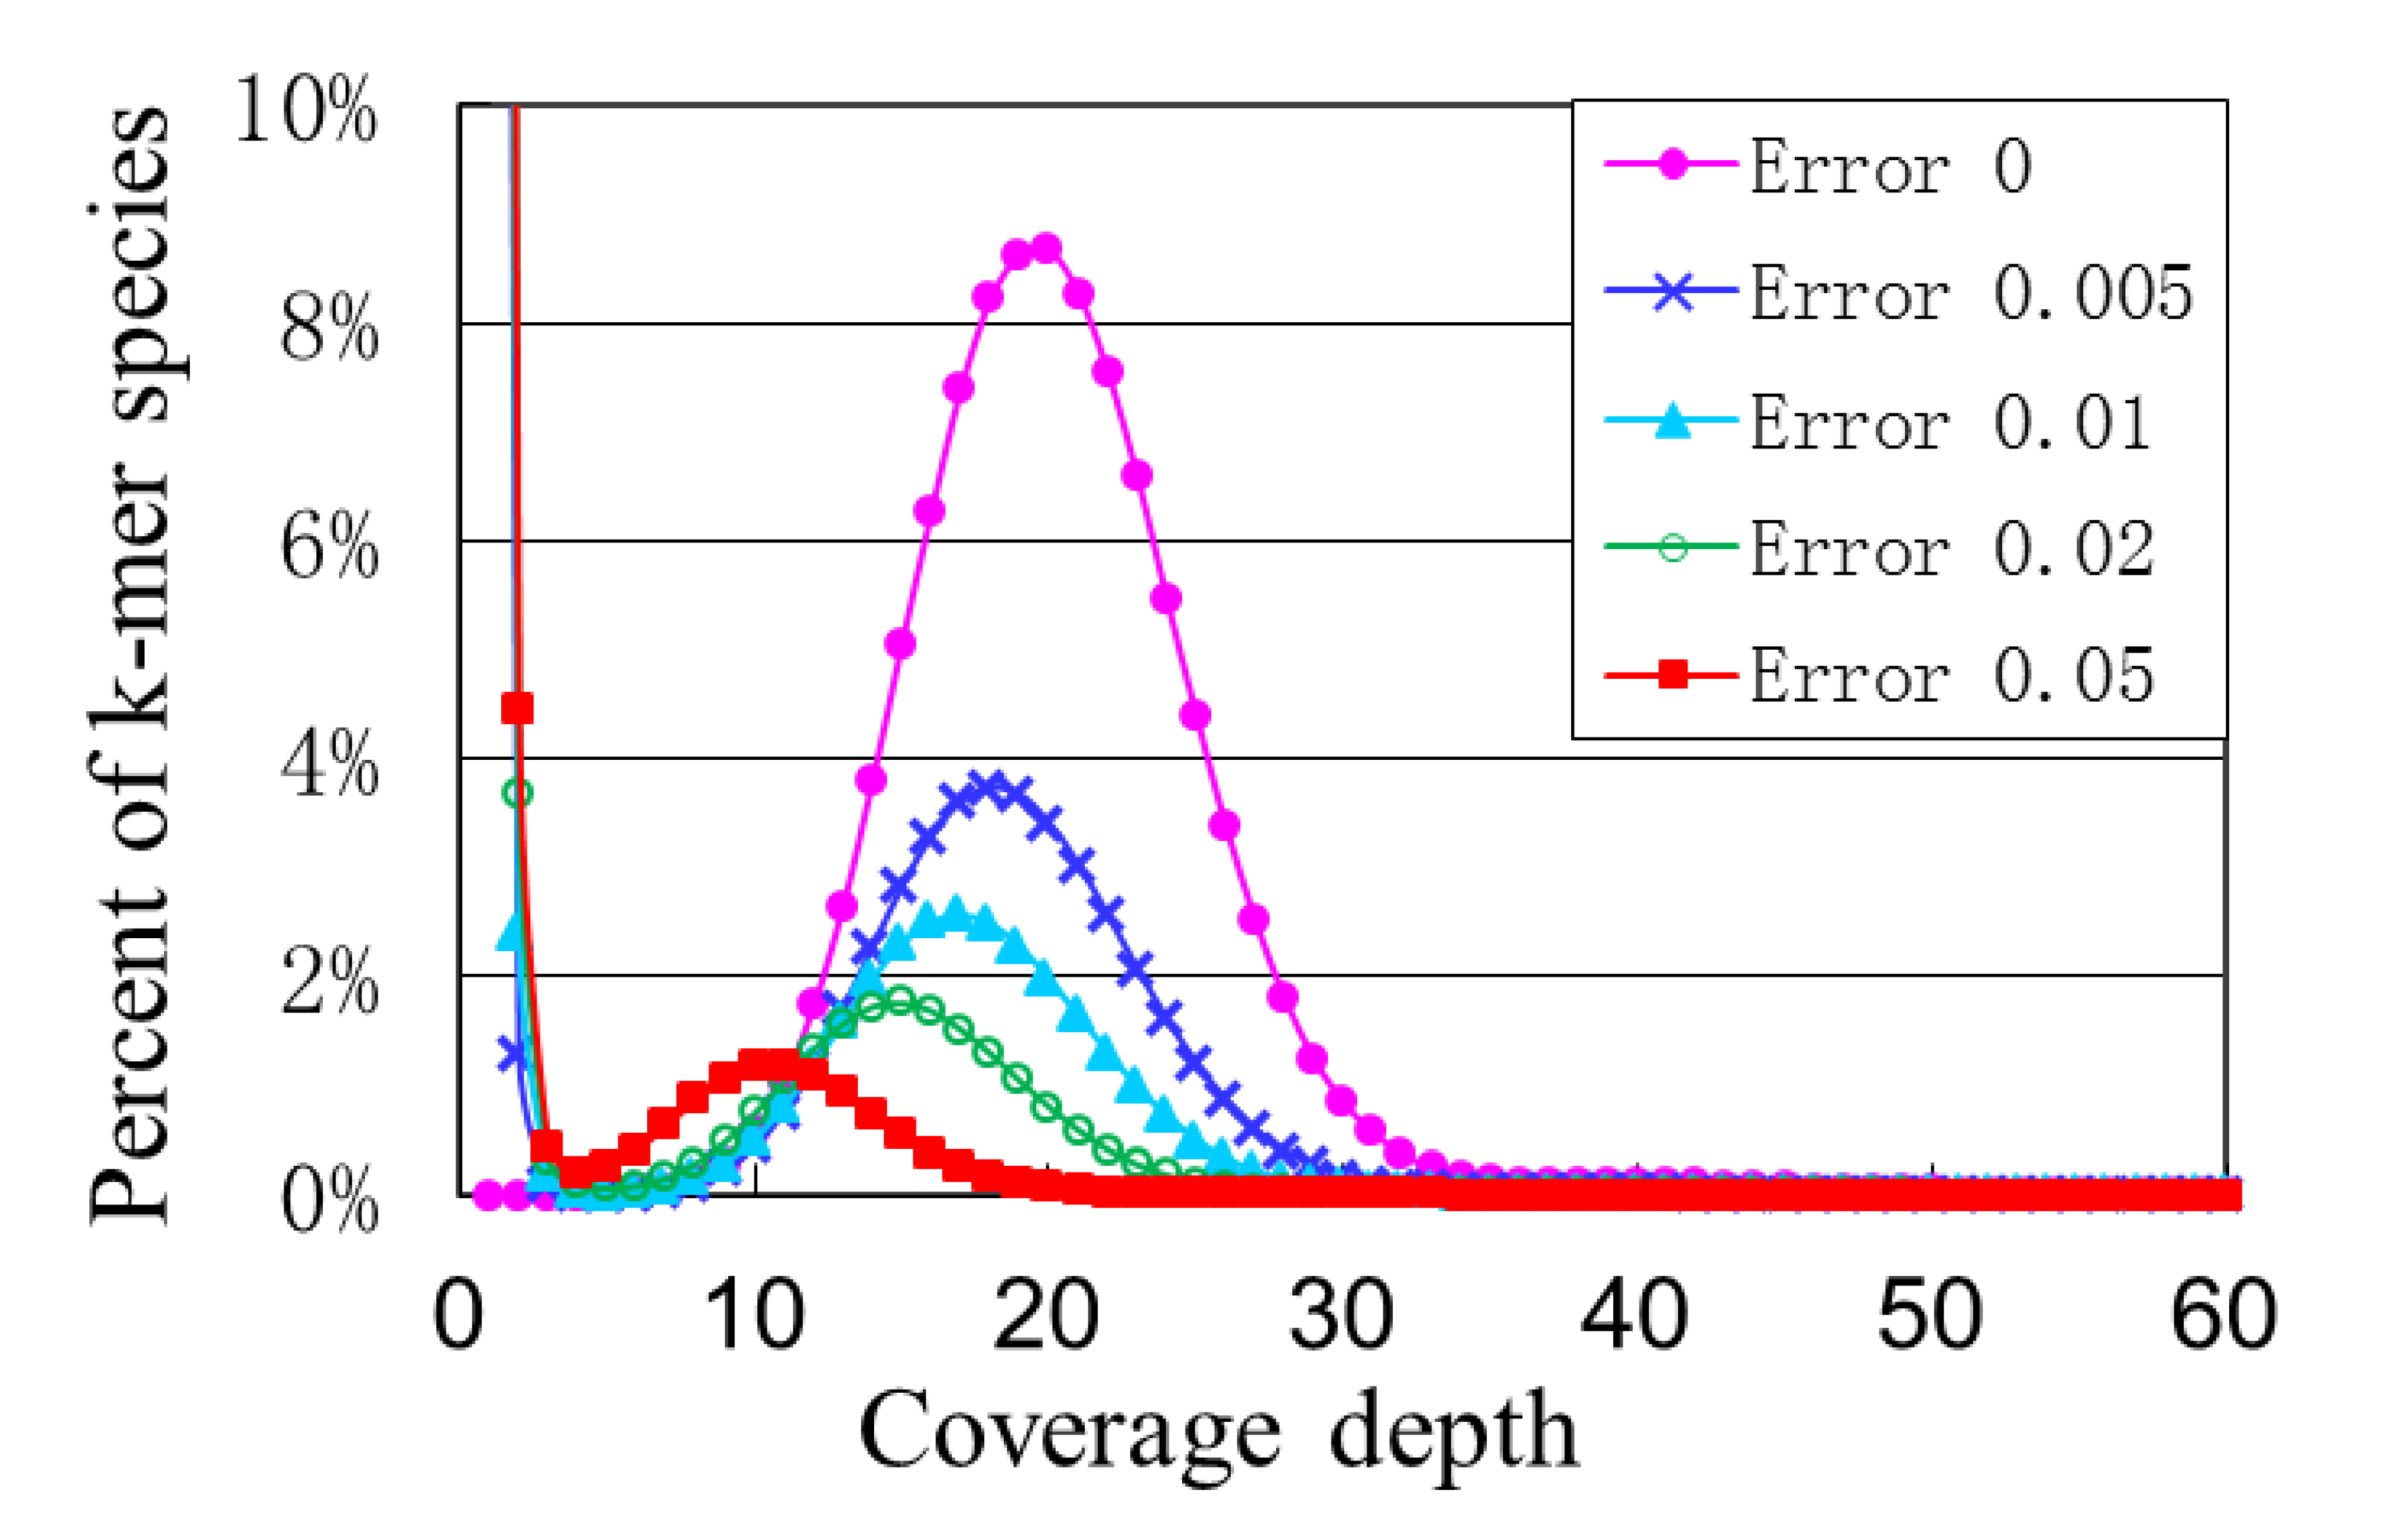
\includegraphics[width=0.48\textwidth]{capitoli/GCE/b.png}} \quad
		\subfloat[][\emph{Grafici degli individui di k-mer, al variare della percentuale di errore.}]
		{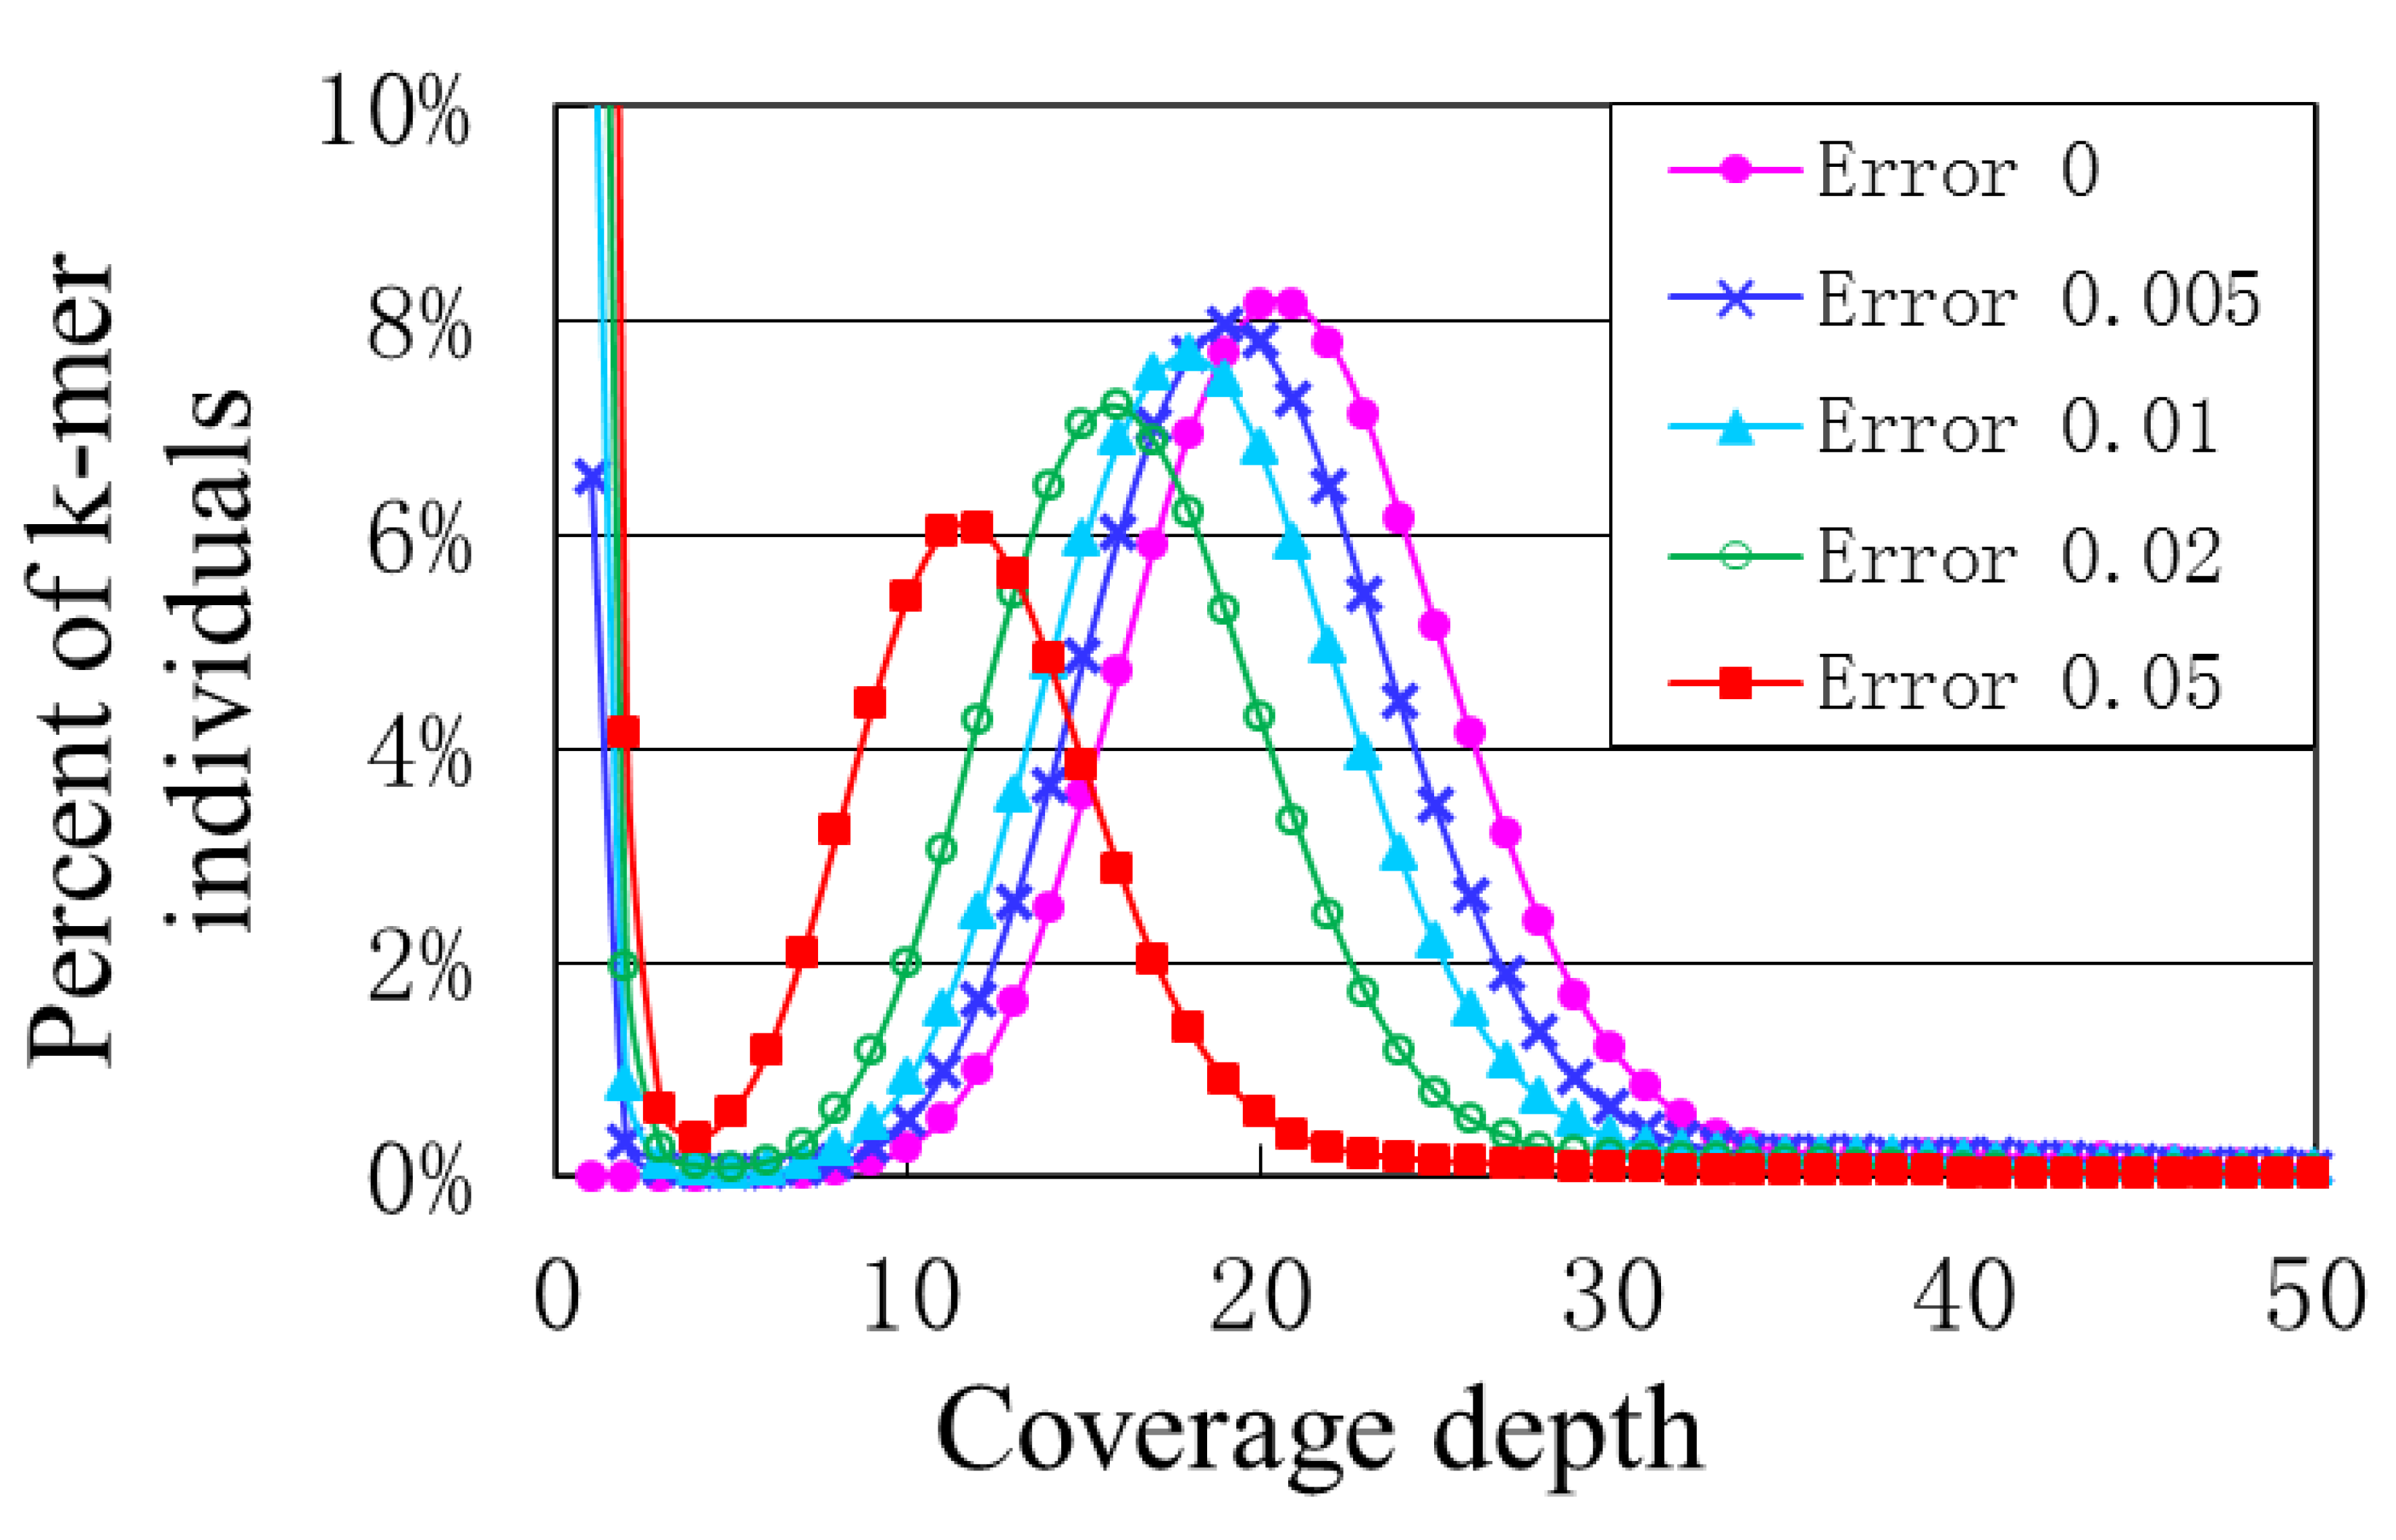
\includegraphics[width=0.48\textwidth]{capitoli/GCE/c.png}} 
		\caption{Effetto degli errori di sequenziamento sui grafici delle specie e degli individui di k-mer. Il picco dei k-mer omozigoti viene appiattito e spostato a sinistra all'aumentare della percentuale di errore.}
		\label{fig:GCEerrors}
	\end{figure}
	
	I \textit{coverage bias}, che corrispondono a deviazioni rispetto alla distribuzione uniforme delle letture~\cite{ross2013characterizing}, sono invece più difficili da gestire, poiché appiattiscono le curve rendendo più difficile l'individuazione dei picchi e la stima di $c$. Anche se in presenza di tali errori i k-mer non vengono campionati in maniera equiprobabile, lo spettro di campionamento risulta continuo. Il nuovo modo di rappresentare le distribuzioni di specie e di individui di k-mer diventa quindi un modello continuo, che viene approssimato con un modello discreto a livelli non uniformi $a_k$, nel quale la copertura $c$ scelta corrisponde al maggior valore $a_k$, mentre il parametro $a_i$ viene stimato come somma dei parametri $a_k$ corrispondenti a ciascun picco. Una volta trovati i valori $c$ e $a_i$, viene stimata la dimensione del genoma tramite la formula~\vref{eqn:GCE2}. 
	
	
\end{document}